%\documentclass[mathserif]{beamer}
\documentclass[handout]{beamer}
%\usetheme{Goettingen}
\usetheme{Warsaw}
%\usetheme{Singapore}
%\usetheme{Frankfurt}
%\usetheme{Copenhagen}
%\usetheme{Szeged}
%\usetheme{Montpellier}
%\usetheme{CambridgeUS}
%\usecolortheme{}
%\setbeamercovered{transparent}
\usepackage[english, activeacute]{babel}
\usepackage[utf8]{inputenc}
\usepackage{amsmath, amssymb}
\usepackage{dsfont}
\usepackage{graphics}
\usepackage{cases}
\usepackage{graphicx}
\usepackage{pgf}
\usepackage{epsfig}
\usepackage{amssymb}
\usepackage{multirow}	
\usepackage{amstext}
\usepackage[ruled,vlined,lined]{algorithm2e}
\usepackage{amsmath}
\usepackage{epic}
\usepackage{epsfig}
\usepackage{fontenc}
\usepackage{framed,color}
\usepackage{palatino, url, multicol}
\usepackage{listings}
%\algsetup{indent=2em}
\newcommand{\factorial}{\ensuremath{\mbox{\sc Factorial}}}
\newcommand{\BIGOP}[1]{\mathop{\mathchoice%
{\raise-0.22em\hbox{\huge $#1$}}%
{\raise-0.05em\hbox{\L
\usepackage{fontenc}
\usepackage{framed,color}
\usepackage{palatino, url, multicol}
\usepackage{listings}
%\algsetup{indent=2em}
\newcommand{\factorial}{\ensuremath{\mbox{\sc Factorial}}}
\newcommand{\BIGOP}[1]{\mathop{\mathchoice%
{\raise-0.22em\hbox{\huge $#1$}}%
{\raise-0.05em\hbox{\Large $#1$}}{\hbox{\large $#1$}}{#1}}}
\newcommand{\bigtimes}{\BIGOP{\times}}
\vspace{-0.5cm}
\title{Introduction to Statistical Inference}
\vspace{-0.5cm}
\author[Felipe Bravo Márquez]{\footnotesize
%\author{\footnotesize  
 \textcolor[rgb]{0.00,0.00,1.00}{Felipe José Bravo Márquez}} 
\date{ \today }
arge $#1$}}{\hbox{\large $#1$}}{#1}}}
\newcommand{\bigtimes}{\BIGOP{\times}}
\vspace{-0.5cm}
\title{Linear Regression}
\vspace{-0.5cm}
\author[Felipe Bravo Márquez]{\footnotesize
%\author{\footnotesize  
 \textcolor[rgb]{0.00,0.00,1.00}{Felipe José Bravo Márquez}} 
\date{ \today }


\begin{document}
\begin{frame}
\titlepage


\end{frame}


%%%%%%%%%%%%%%%%%%%%%%%%%%%



\begin{frame}{Introduction}
\scriptsize{
\begin{itemize}

 \item  A regression model is used to model the relationship of a numerical dependent variable $\mathbf{y}$ with $m$ independent variables  $\mathbf{x}_1, \mathbf{x}_2, \dots, \mathbf{x}_m$ \cite{wasserman2013all}. 
 
 \item The dependent variable $\mathbf{y}$ is also called \textbf{target}, \textbf{outcome}, or \textbf{response} variable.
 
 \item The independent variables  $\mathbf{x}_1, \mathbf{x}_2, \dots, \mathbf{x}_m$ are also called \textbf{covariates}, \textbf{attributes}, \textbf{features}, por \textbf{predictor variables}.
 
 
 \item  Roughly speaking we want to know the expected value of $\mathbf{y}$ from the values of $\mathbf{x}$:
 \begin{displaymath}
 \mathbb{E}(y|x_1,x_2,\dots,x_m)
 \end{displaymath}

 
 \item  We use these models when we believe that the response variable $\mathbf{y}$ can be modeled by other independent variables.
 
 \item To perform this type of analysis we need a dataset consisting of $n$ observations that include both the response variable and each of the attributes.
 
 \item We refer to the process of \textbf{fitting} a regression function as the process in which from the data we infer a hypothesis function $h$ that allows us to \textbf{predict} unknown $\mathbf{y}$ values using the values of the attributes.

 
\end{itemize}



} 
 
\end{frame}


\begin{frame}{Introduction (2)}
\scriptsize{
\begin{itemize}
 
 \item This process of fitting a function from data is referred to in the areas of data mining and machine learning as \textbf{training}.

 \item In those disciplines, functions are said to \textbf{learn} from data.
 
 \item Since we need observations where the value of $\mathbf{y}$ is known to learn the function, such techniques are referred to as \textbf{supervised learning} techniques.
 
 \item When $\mathbf{y}$ is a categorical variable we have a \textbf{classification} problem. 
 

 
\end{itemize}


\begin{figure}[h!]
	\centering
	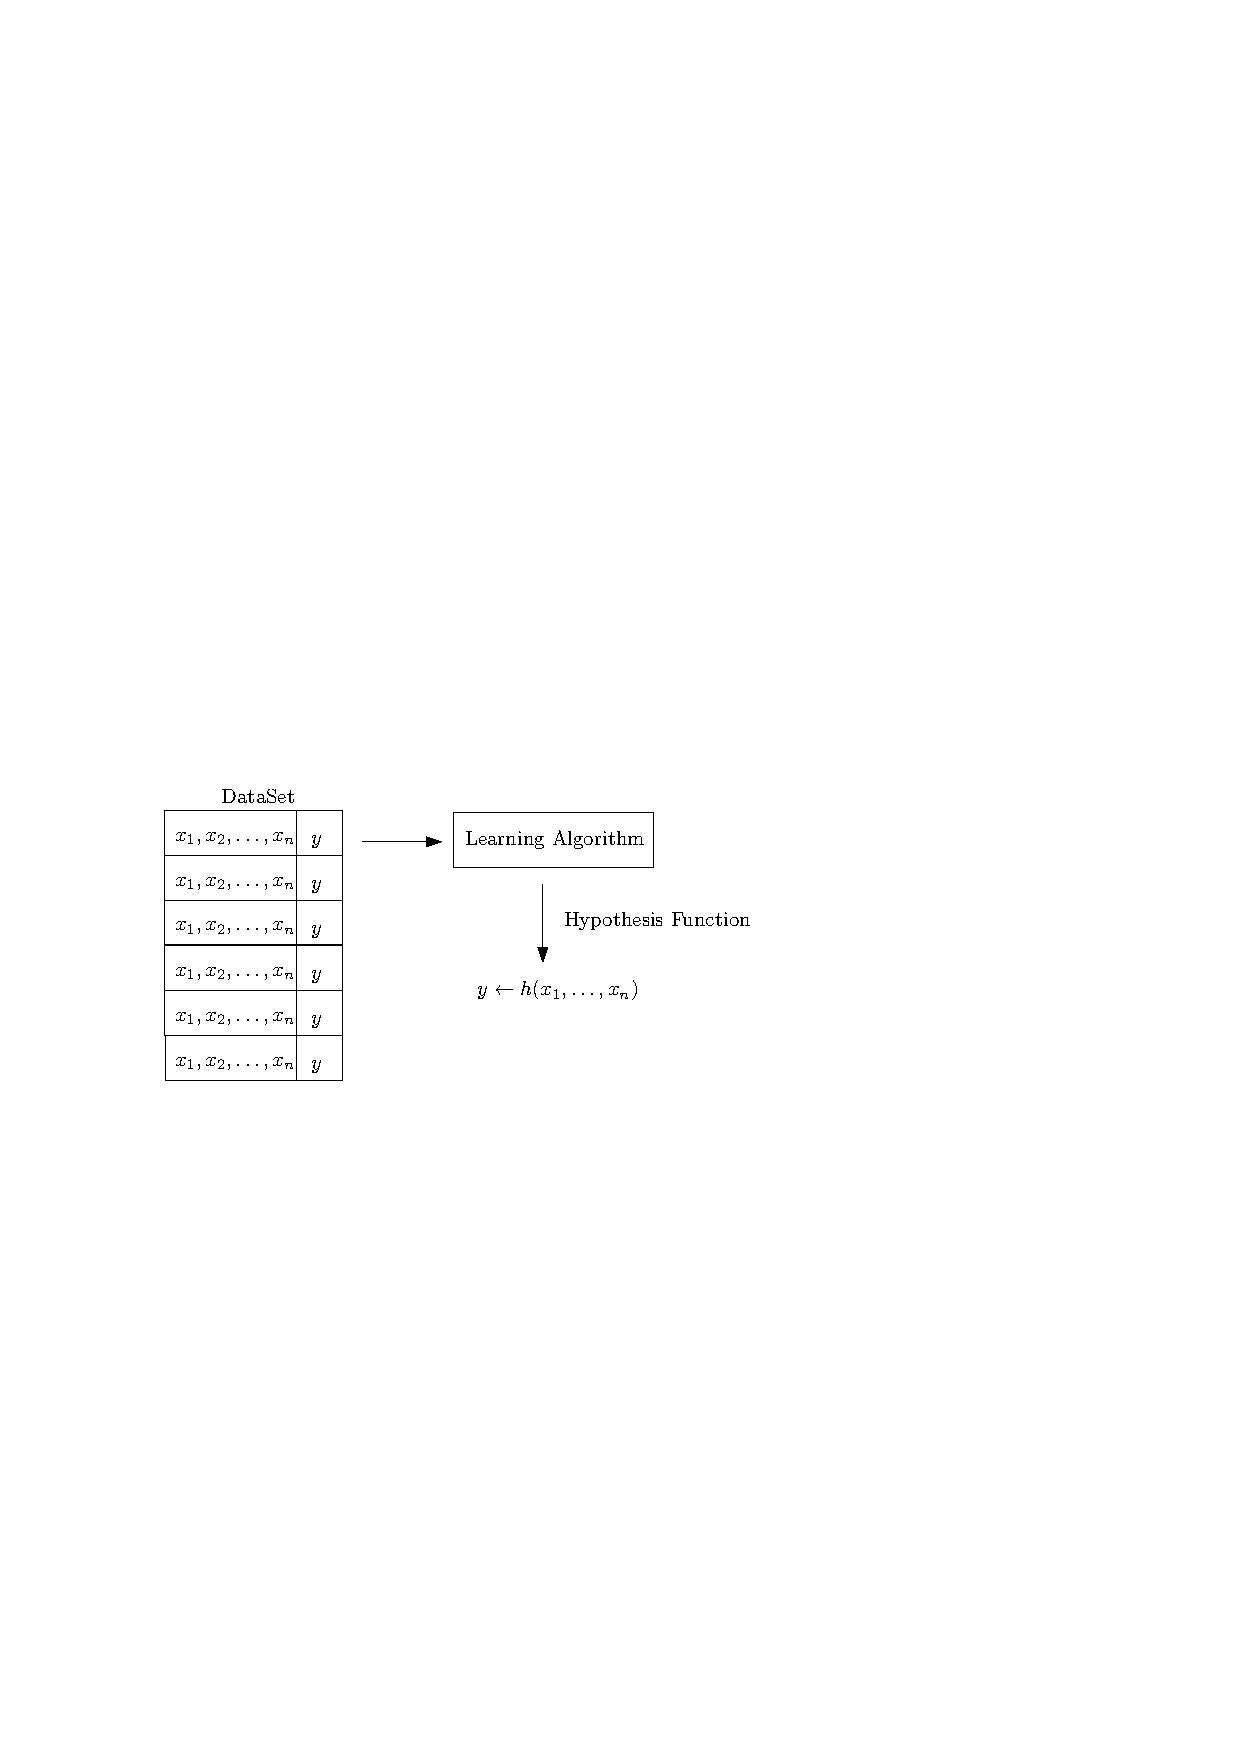
\includegraphics[scale=0.4]{pics/learning.pdf}
\end{figure}

} 
 
\end{frame}


\begin{frame}{Simple Linear Regression}
\scriptsize{
\begin{itemize}
 \item In simple linear regression, we have a single independent variable $x$ to model the dependent variable $\mathbf{y}$.

 \item The following linear relationship between the variables is assumed:

\begin{displaymath}
 y_i=\beta_{0}+\beta_{1}x_i +\epsilon_i \quad \forall i
\end{displaymath}

\item The parameter $\beta_{0}$ represents the intercept of the line (the value of $y$ when $x$ is zero).  

\item The parameter $\beta_{1}$ is the slope and represents the change of $\mathbf{y}$ when we vary the value of $\mathbf{x}$. The greater the magnitude of this parameter the greater the linear relationship between the variables.

\item The $\epsilon_{i}$ values correspond to the errors or \textbf{residuals} associated with the model.

\item We have to find a linear function or straight line $h_\beta$ that allows us to find an estimate of $y$, $\hat{y}$ for any value of $x$ with the minimum expected error.

\begin{displaymath}
h(x)=\beta_{0}+\beta_{1}x 
\end{displaymath}


\end{itemize}


} 
 
\end{frame}



\begin{frame}{Simple Linear Regression}
\scriptsize{

\begin{figure}[h!]
	\centering
	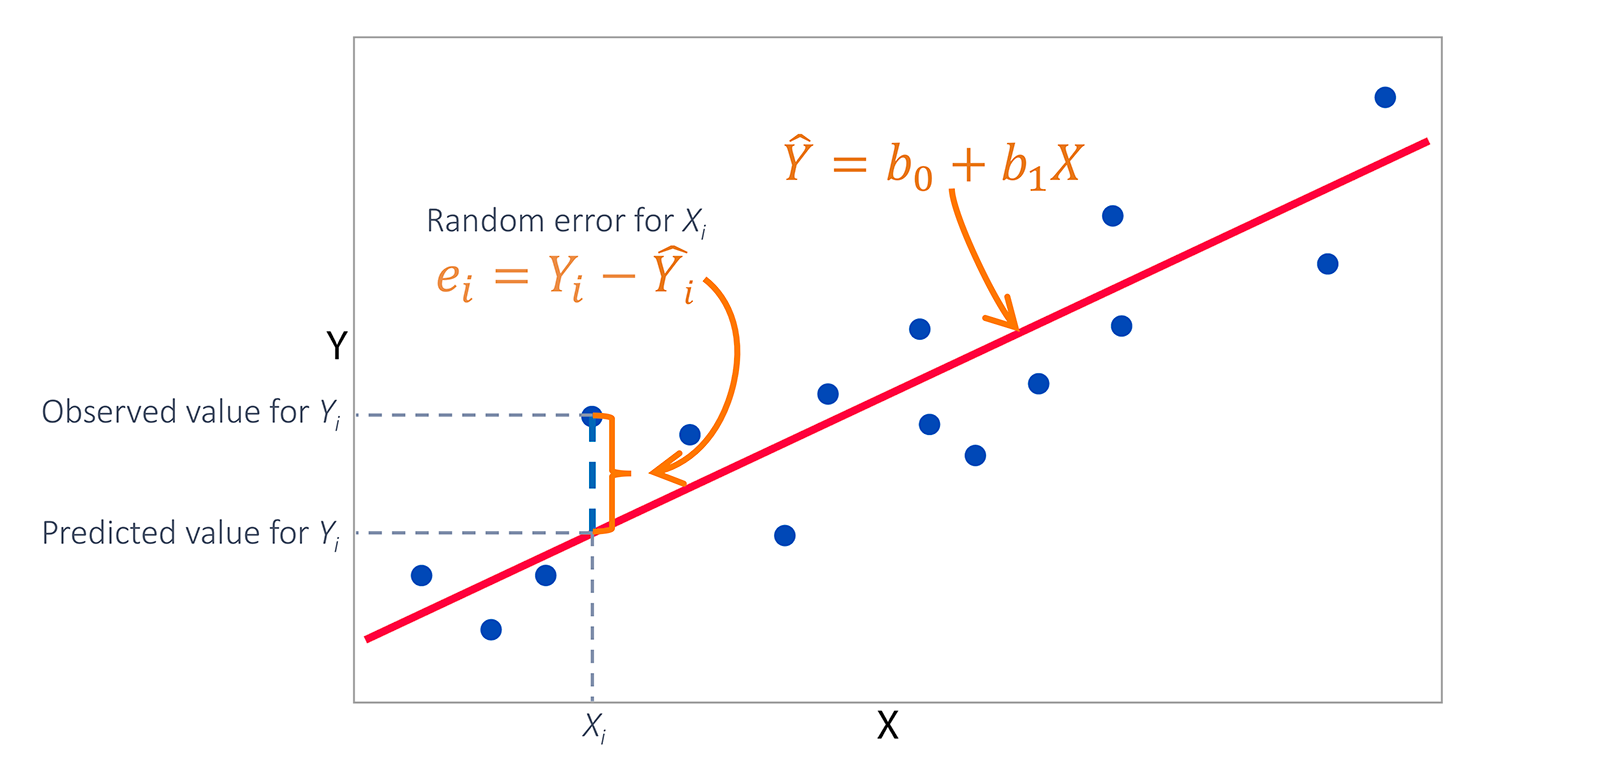
\includegraphics[scale=0.21]{pics/linear_model.png}
	\caption{Source: \url{https://www.jmp.com}}
\end{figure}

} 
 
\end{frame}


\begin{frame}{Least Squares}
\scriptsize{
\begin{itemize}

 \item The ordinary least squares method is used to estimate  $\hat{\beta}_{0}$ and $\hat{\beta}_{1}$ by minimizing the sum of squared errors (SSE) of the observed data.

 \item Suppose we have $n$ observations of $\mathbf{y}$ and $\mathbf{x}$, we compute the sum of squared errors (SSE) as follows:

\begin{equation}
SSE = \sum_{i=1}^{n} (y_i-h(x_i))^2 =  \sum_{i=1}^{n} (y_i-\beta_{0}-\beta_{1}x_i)^2
\end{equation}

 \item To find the parameters that minimize the error we calculate the partial derivatives of SSE with respect to $\beta_{0}$ and $\beta_{1}$. Then we equal the derivatives to zero and solve the equation to find the parameter values.
 
 \begin{equation}
 \frac{\partial SSE}{ \partial \beta_0} = -2\sum_{i=1}^{n}(y_i-\beta_{0}-\beta_{1}x_i)=0
 \end{equation}

  \begin{equation}
 \frac{\partial SSE}{ \partial \beta_1} = -2\sum_{i=1}^{n}(y_i-\beta_{0}-\beta_{1}x)x_i=0
 \end{equation}



\end{itemize}



} 
\end{frame}

\begin{frame}{Least Squares (2)}
\scriptsize{
\begin{itemize}
 \item From the above system of equations the normal solutions are obtained:
  \begin{equation}
 \hat{\beta}_{1} = \frac{\sum_{i}^{n} (x_i-\overline{x})(y_i-\overline{y}) }{ \sum_{i}^{n} (x_i-\overline{x})^2}    
 \end{equation}

 \begin{equation}
 \hat{\beta}_{0} = \overline{y} -\hat{\beta}_{1}\overline{x}    
 \end{equation}



\item The fitted model represents the line of least squared error.

\begin{figure}[h!]
	\centering
	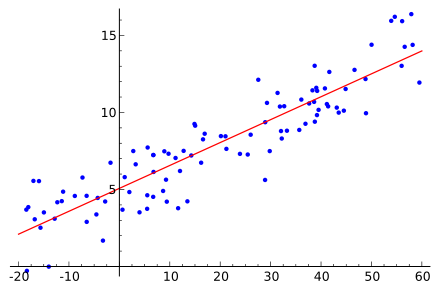
\includegraphics[scale=0.35]{pics/Linear_regression.png}
\end{figure}

\end{itemize}

} 
 
\end{frame}


\begin{frame}{Coefficient of Determination $R^2$}
\scriptsize{
\begin{itemize}
 \item  Once we have fitted our linear model we must evaluate the quality of the model.
 \item A very common metric is the coefficient of determination $R^2$. 
 \item  It is calculated from errors that are different than the SSE squared errors.
 \item The total sum of squares (SST)  is defined as the predictive error when we use the mean $\overline{y}$  to predict the response variable $y$ (it is very similar to the variance of the variable):
 \begin{displaymath}
  \text{SST} = \sum_{i}^{n}(y_i-\overline{y})^2  
 \end{displaymath}
 \item  The regression sum of squares (SSM), on the other hand, represents the amount of error in the regression model: 

 \begin{displaymath}
  \text{SSM} = \sum_{i}^{n}(\hat{y}_i-\overline{y})^2 
 \end{displaymath}
  
 \item  SSM indicates the variability of the values predicted by the model with respect to the mean. 
 
  
\end{itemize}

}
\end{frame}

\begin{frame}{Coefficient of Determination $R^2$ (2)}
\scriptsize{
\begin{itemize}
 \item It can be proved that all the above errors are related as follows: \begin{equation}
 SST = SSE + SSM                                                 
    \end{equation}


 \item The coefficient of determination for a linear model $R^2$ is defined as:
 \begin{equation}
  R^2= \frac{\text{SSM}}{\text{SST}} = \frac{\sum_{i}^{n}(\hat{y}_i-\overline{y})^2 }{\sum_{i}^{n}(y_i-\overline{y})^2  }
 \end{equation}
 
 \item An alternative but equivalent definition:
  \begin{equation}
  R^2= 1-\frac{\text{SSE}}{\text{SST}} = 1- \frac{\sum_{i}^{n}(y_i-\hat{y}_i)^2 }{\sum_{i}^{n}(y_i-\overline{y})^2  }
  \label{eq:r2}
 \end{equation}
 

  
\end{itemize}


}
\end{frame}




\begin{frame}{Coefficient of Determination $R^2$ (2)}
\scriptsize{
\begin{itemize}
 
 \item Another alternative but equivalent definition:
 
   \begin{equation}
  R^2= 1-\frac{\text{var}(\epsilon)}{\text{var}(y)} 
 \end{equation}

 \item It is often interpreted as the ``variance explained'' by the model.
 
 \item The coefficient usually takes values between $0$ to $1$ and the closer its value is to 1 the higher the quality of the model\footnote{It can take negative values when predictions are worse than using $\overline{y}$ in all predictions.}.
 
 \item The value of $R^2$ is equivalent to the squared linear correlation (Pearsons) between $y$ and $\hat{y}$.
\begin{displaymath}
 R^2=\text{cor}(y,\hat{y})^2
\end{displaymath}
  
\end{itemize}


}
\end{frame}



\begin{frame}{Assumptions of the Linear Model}
\scriptsize{





Whenever we fit a linear model we are implicitly making certain assumptions about the data.  


\begin{block}{Assumptions}
\begin{enumerate}
\item Linearity: the response variable is linearly related to the attributes. 
\item  Normality: errors have a zero mean normal distribution: $\epsilon_{i} \sim N(0,\sigma^2)$.
\item Homoscedasticity: errors have constant variance (same value of $\sigma^2$).
\item Independence: errors are independent of each other.
 
\end{enumerate}
 
\end{block}

} 
\end{frame}


\begin{frame}{Probabilistic Interpretation}
\scriptsize{
\begin{itemize}
 \item Considering the above assumptions, we are saying that the probability density (PDF) of the errors $\epsilon$ is defined by a normal of zero mean and constant variance:
 \begin{displaymath}
  \text{PDF}(\epsilon_{i})=\frac{1}{\sqrt{2\pi} \sigma} \exp \left(- \frac{\epsilon_{i}^{2}}{2\sigma^2}\right)
 \end{displaymath}
 \item Moreover all $\epsilon_{i}$ are IID (independent and identically distributed).
 \item This implies that:
  \begin{displaymath}
  \text{PDF}(y_i|x_{i};\beta)=\frac{1}{\sqrt{2\pi} \sigma} \exp \left(- \frac{(y_i - h_{\beta}(x_{i}) )^{2}}{2\sigma^2}\right)
 \end{displaymath}
\item Which implies that the distribution of $\mathbf{y}$ given the values of $\mathbf{x}$ and parameterized by $\beta$ follows a normal distribution.

\item Let's estimate the parameters of the model  ($\beta$) using maximum likelihood estimation.

\end{itemize}

}
 
\end{frame}


\begin{frame}{Probabilistic Interpretation}
\scriptsize{
\begin{itemize}



 \item The likelihood function of $\beta$ can be written as:
 
 \begin{displaymath}
  \mathcal{L}(\beta) = \prod_{i=1}^{n}\frac{1}{\sqrt{2\pi} \sigma} \exp \left(- \frac{(y_i - h_{\beta}(x_{i}) )^{2}}{2\sigma^2}\right)
 \end{displaymath}

 \item and the the log likelihood $l_n(\beta)$:
 
   \begin{align}
l_n(\beta)  & =  \log  \mathcal{L}(\beta) \\
 & = \log \prod_{i=1}^{n}\frac{1}{\sqrt{2\pi} \sigma} \exp \left(- \frac{(y_i - h_{\beta}(x_{i}) )^{2}}{2\sigma^2}\right) \\
  & = \sum_{i=1}^n  \log \prod_{i=1}^{n}\frac{1}{\sqrt{2\pi} \sigma} \exp \left(- \frac{(y_i - h_{\beta}(x_{i}) )^{2}}{2\sigma^2}\right) \\
    & = n \log\left(\frac{1}{\sqrt{2\pi} \sigma}\right) - \frac{1}{\sigma^2}\times \frac{1}{2}\sum_{i=1}^n(y_i - h_{\beta}(x_{i}) )^{2}  
 \end{align}
 

\end{itemize}


}
 
\end{frame}


\begin{frame}{Probabilistic Interpretation}
\scriptsize{
\begin{itemize}



 \item Hence, maximizing $l_n(\beta)$ gives the same answer as minimizing
 
 \begin{displaymath}
\sum_{i=1}^n(y_i - h_{\beta}(x_{i}))^{2}
 \end{displaymath}

 \item which is equivalent as minimizing SSE.
 
 \item  Then, if one estimates the parameters of $\beta$ using maximum likelihood estimation one arrives at the same results as doing least squares estimation.
 \item This tells us that when we estimate the model parameters using least squares we are making the same probabilistic assumptions mentioned above.

\end{itemize}


}
 
\end{frame}



\begin{frame}{Standard errors for regression models}
\scriptsize{
\begin{itemize}
 \item If we want to make inferences about the regression parameter estimates, then we also need an estimate of their variability. \cite{poldrack2019statistical}
 \item To compute this, we first need to compute the residual variance or error variance for the model.
 \item That is, how much variability in the dependent variable is not explained by the model. 
 \item We need to compute the mean squared error:
 
 \begin{displaymath}
  MS_{error} = \frac{SSE}{df} = \frac{\sum_{i=1}^{n} (y_i-h(x_i))^2}{n-p}
 \end{displaymath}

 \item The degrees of freedom ($df$) are determined by subtracting the number of estimated parameters (2 in this case: $\beta_0$ and $\beta_1$) from the number of observations ($n$)

 \item  We can compute the standard error for the model as: $SE_{model} = \sqrt{MS_{error}}$
 


 
\end{itemize}


}
 
\end{frame}



\begin{frame}{A significance test for $\beta$}
\scriptsize{
\begin{itemize}

 \item In order to get the standard error for a specific regression parameter estimate, $SE_{\beta_x}$, we need to rescale the standard error of the model by the square root of the sum of squares of the X variable:
 
 \begin{displaymath}
  SE_{\hat{\beta}_x} = \frac{SE_{model}}{\sqrt{\sum_{i=1}^n(x_i-\overline{x})^2}}
   \end{displaymath}


  \item Now we can compute a $t$ statistic to tell us the likelihood of the observed parameter estimates compared to some expected value under the null hypothesis. 
   
 \item In this case we will test against the null hypothesis of no effect (i.e. $\beta_{H_0}=0$):
 
 \begin{displaymath}
  t_{n-p} = \frac{\hat{\beta}-\beta_{H_0}}{ SE_{\hat{\beta}_x}} = \frac{\hat{\beta}}{ SE_{\hat{\beta}_x}}
 \end{displaymath}

 \item Later we will see that R automatically reports the t-statistics and p-values of all coefficients of a linear model.
 
 \item This allows us to determine whether the linear relationship between the two variables ($y$ and $x$) is significant.
 
\end{itemize}


}
 
\end{frame}


\begin{frame}[fragile]{Example: a model of height}
\scriptsize{
\begin{itemize}
 \item  We are going to work with the dataset \verb+Howell1+ that has demographic data from Kalahari !Kung San people collected by Nancy Howell in the late 1960s. 
 \item The !Kung San are the most famous foraging population of the twentieth century, largely because of detailed quantitative studies by people like Howell. \cite{mcelreath2020statistical}
 \end{itemize} 

 
 \begin{figure}[h!]
	\centering
	
\includegraphics[scale=0.6]{pics/San_Schmuck.jpg}
	\caption{By Staehler - Own work, CC BY-SA 4.0, \url{https://commons.wikimedia.org/w/index.php?curid=45076017}}
\end{figure}

 
}
\end{frame}


\begin{frame}[fragile]{Example: a model of height}
\scriptsize{
\begin{itemize}
 \item Each observation corresponds to an individual.
 \item The variables of the dataset are:
 \begin{enumerate}
 \scriptsize{
\item height: height in cm
\item weight: weight in kg
\item age: age in years
\item male: gender indicator (1 for male 0 for woman)
  }
 \end{enumerate}
 
\item Let's explore the linear correlations between the variables

 \begin{verbatim}
> d <- read.csv("howell1.csv")
> cor(d)
          height    weight         age        male
height 1.0000000 0.9408222 0.683688567 0.139229021
weight 0.9408222 1.0000000 0.678335313 0.155442866
age    0.6836886 0.6783353 1.000000000 0.005887126
male   0.1392290 0.1554429 0.005887126 1.000000000
 \end{verbatim}

 
 
 
\end{itemize}
 
 
 
 
} 
\end{frame}


\begin{frame}[fragile]{Example: a model of height}
\scriptsize{
\begin{itemize}
 \item We can see that there is a positive correlation between \verb+height+ and \verb+age+.
 
 \item Let's filter out the non-adult examples because we know that height is strongly correlated with age before adulthood. 
 
  \begin{verbatim}
   d2 <- d[ d$age >= 18 , ]
  \end{verbatim}

 \item Now age doesn't correlate with height:
 

  \begin{verbatim}
> cor(d2)
           height     weight         age       male
height  1.0000000  0.7547479 -0.10183776 0.69999340
weight  0.7547479  1.0000000 -0.17290430 0.52445271
age    -0.1018378 -0.1729043  1.00000000 0.02845498
male    0.6999934  0.5244527  0.02845498 1.00000000
  \end{verbatim} 
 
 
 \item Let's model height as a function of weight using a simple linear regression:
 \begin{displaymath}
  \text{height}(\text{weight})=\beta_0+\beta_1*\text{weight}
 \end{displaymath}
 

 
 

 
 


\end{itemize}
 
 
 
} 
\end{frame}

\begin{frame}[fragile]{Example: a model of height}
\scriptsize{



\begin{itemize}

  \item In R the linear models are created with the command \verb+lm+ that receives as parameter a formula of the form \verb+y~x+ ($y=f(x)$).

\begin{verbatim}
> reg1<-lm(height~weight,d2)
> reg1

Call:
lm(formula = height ~ weight, data = d2)

Coefficients:
(Intercept)       weight  
    113.879        0.905  
\end{verbatim}



 
 \end{itemize}
 
 


} 
\end{frame}


\begin{frame}[fragile]{Example: a model of height}
\scriptsize{

 \begin{itemize}
 
  \item We can see that the coefficients of the model are $\beta_{0}=113.879$ and $\beta_{1}=0.905$. 


\item The estimate of $\beta_{0}=113.879$, indicates that a person of weight 0 should be around $114$cm tall, which we know is nonsense but it what our linear model believes.  
 
 \item Since $\beta_1$ is a slope, the value $0.905$ can be read as a person 1 kg heavier is expected to be 0.90 cm taller.
 
 
 \item We can directly access the coefficients and store them in a variable:
 \begin{verbatim}
> reg1.coef<-reg1$coefficients
> reg1.coef
(Intercept)      weight 
113.8793936   0.9050291 
 \end{verbatim}

 
 \end{itemize}
 
 


} 
\end{frame}


\begin{frame}[fragile]{Example: a model of height}
\scriptsize{


\begin{itemize}


\item We can view various indicators about the linear model with the command \textbf{summary}:
 
\begin{verbatim}
> summary(reg1)

Call:
lm(formula = height ~ weight, data = d2)

Residuals:
     Min       1Q   Median       3Q      Max 
-19.7464  -2.8835   0.0222   3.1424  14.7744 

Coefficients:
             Estimate Std. Error t value Pr(>|t|)    
(Intercept) 113.87939    1.91107   59.59   <2e-16 ***
weight        0.90503    0.04205   21.52   <2e-16 ***
---
Signif. codes:  0 ‘***’ 0.001 ‘**’ 0.01 ‘*’ 0.05 ‘.’ 0.1 ‘ ’ 1

Residual standard error: 5.086 on 350 degrees of freedom
Multiple R-squared:  0.5696,	Adjusted R-squared:  0.5684 
F-statistic: 463.3 on 1 and 350 DF,  p-value: < 2.2e-16

\end{verbatim}
\item We can see that $\beta_0$ and $\beta_1$ are both statistically significantly different from zero.  
 
 \end{itemize}
 
 


} 
\end{frame}




\begin{frame}[fragile]{Example: a model of height}
\scriptsize{
\begin{itemize}
 \item We see that the coefficient of determination $R^2$ has a value of $0.57$ which is not so good but acceptable.
 
 
  \item We can conclude that the weight while providing useful information to model a part of the variability of the height of the !Kung people, is not enough to build a highly reliable model. 
  
  \item We can store the results of the command \verb+summary+ in a variable then access the coefficient of determination:
\begin{verbatim}
> sum.reg1<-summary(reg1)
> sum.reg1$r.squared
[1] 0.5696444  
\end{verbatim}

\item  We can also access the fitted values which are the values predicted by my model for the data used:
\begin{verbatim}
> reg1$fitted.values
       1        2        3        4        5        6      
157.1630 146.9001 142.7180 161.8839 151.2362 170.8895 
\end{verbatim}
 
 \end{itemize}
 

} 
\end{frame}



\begin{frame}[fragile]{Example: a model of height}
\scriptsize{
\begin{itemize}
 \item We can check now that all definitions given for $R^2$ are equivalent.
 
 \begin{verbatim}
> SSE<-sum(reg1$residuals^2)
> SST<-sum((d2$height-mean(d2$height))^2)
> SSM<-sum((reg1$fitted.values-mean(d2$height))^2)
> SSM/SST
[1] 0.5696444
> 1-SSE/SST
[1] 0.5696444
> 1-var(reg1$residuals)/var(d2$height)
[1] 0.5696444
> cor(d2$height,reg1$fitted.values)^2
[1] 0.5696444
 \end{verbatim}

 
 \end{itemize}
 

} 
\end{frame}


\begin{frame}[fragile]{Example: a model of height}
\scriptsize{
\begin{itemize}
\item  Suppose now that we know the weight for two !Kung people but we don't know their height.

\item  We could use our linear model to predict the height of these two people.

\item To do this in R we must use the command \verb+predict.lm+ which receives the linear model and a data.frame with the new data:
\begin{verbatim}
> new.weights<-data.frame(weight=c(50,62))
> predict.lm(object=reg1,newdata=new.weights)
       1        2 
159.1308 169.9912 
> # this is equivalent to:
> reg1.coef[1]+reg1.coef[2]*new.weights[1:2,]
[1] 159.1308 169.99122
\end{verbatim}

 
 \end{itemize}
 

} 
\end{frame}


\begin{frame}{Multivariate Linear Regression}
\scriptsize{
\begin{itemize}
 \item Suppose we have $m$ independent variables:  $x_1,x_2,\dots,x_m$.
 \item In many cases more variables can better explain the variability of the response variable $\mathbf{y}$ than a single one.
 \item A multivariate linear model is defined as follows:
 \begin{displaymath}
 y_i=\beta_{0}+\beta_{1}x_{i,1}+ +\beta_{2}x_{i,2} + \cdots + \beta_{m}x_{i,m} +  \epsilon_i \quad \forall i \in \{1,n\}
\end{displaymath}

\item In essence we are adding a parameter for each independent variable.

\item Then, we multiply the parameter by the variable and add that term to the linear model.

\item  In the multivariate model all the properties of the simple linear model are extended.

\item The problem can be represented in a matrix form:
\begin{displaymath}
 Y=X\beta+\epsilon
\end{displaymath}








\end{itemize}
 

}
\end{frame}

\begin{frame}{Multivariate Linear Regression (2)}
\scriptsize{
\begin{itemize} 
\item Where $Y$ is a vector $n\times 1$ response variables:

\begin{displaymath}
 Y =
 \begin{pmatrix}
  y_{1} \\
  y_{2}  \\
  \vdots  \\
  y_{n}
 \end{pmatrix}
\end{displaymath}

\item $X$ is a $n \times (m+1)$  matrix with the explanatory variables. We have $n$ observations of the $m$ variables.  The first column is constant equal to $1$ ($x_{i,0}=1 \quad \forall i$) to model the intercept variables $\beta_0$.

\begin{displaymath}
 X =
 \begin{pmatrix}
x_{1,0} &  x_{1,1} & x_{1,2} & \cdots & x_{1,m} \\
x_{2,0} &  x_{2,1} & x_{2,2} & \cdots & x_{2,m} \\
\vdots  &  \vdots  & \vdots  & \ddots & \vdots  \\
x_{n,0} &  x_{n,1} & x_{n,2} & \cdots & x_{n,m}
 \end{pmatrix}
\end{displaymath}






\end{itemize}
 

}
\end{frame}

\begin{frame}{Multivariate Linear Regression (2)}
\scriptsize{
\begin{itemize}
 \item Then, $\beta$ is a $(m+1) \times 1$ vector of parameters.

\begin{displaymath}
 \beta =
 \begin{pmatrix}
  \beta_{0}  \\
  \beta_{1}  \\
  \vdots    \\
  \beta_{m} 
 \end{pmatrix}
\end{displaymath}


\item Finally, $\epsilon$  is a $n \times 1$ vector with the model errors. 

\begin{displaymath}
 \epsilon =
 \begin{pmatrix}
  \epsilon_{1}  \\
  \epsilon_{2}  \\
  \vdots    \\
  \epsilon_{n} 
 \end{pmatrix}
\end{displaymath}

\item  Using matrix notation, we can see that the sum of squared errors (SSE) can be expressed as:
\begin{displaymath}
 \text{SSE} = (Y - X\beta)^{T}(Y-X\beta)
\end{displaymath}

\item Minimizing this expression by deriving the error as a function of $\beta$ and setting it equal to zero leads to the normal equations:

\begin{displaymath}
   \hat{\beta} = (X^{T}X)^{-1} X^{T}Y
\end{displaymath}


\end{itemize}


}

\end{frame}





\begin{frame}[fragile]{Multivariate Linear Regression in R}
\scriptsize{
\begin{itemize}
 \item  Now we will study a multiple linear regression for the \verb+Howell1+ data.
 \item Let's add the variable \textbf{age} as an additional predictor for \textbf{height}.
 \item We know that age is good at predicting height for non-adults so we will work with the original dataset.
 \item  Let's fit the following linear multi-variate model:
 \begin{displaymath}
 \text{height}(\text{weight,age})=\beta_{0}+\beta_{1}*\text{weight}+\beta_{2}*\text{age}
 \end{displaymath}
 \item In R, we add more variables to the linear model with the operator \textbf{+} :
\begin{verbatim}
reg2<-lm(height~weight+age,d)
\end{verbatim}



 
 \end{itemize}
 

} 
\end{frame}


\begin{frame}[fragile]{Multivariate Linear Regression in R (7)}
\scriptsize{

\begin{verbatim}
> summary(reg2)

Call:
lm(formula = height ~ weight + age, data = d)

Residuals:
     Min       1Q   Median       3Q      Max 
-29.0350  -5.4228   0.7333   6.4919  19.6964 

Coefficients:
            Estimate Std. Error t value Pr(>|t|)    
(Intercept) 75.96329    1.04216  72.890  < 2e-16 ***
weight       1.65710    0.03656  45.324  < 2e-16 ***
age          0.11212    0.02594   4.322 1.84e-05 ***
---
Signif. codes:  0 ‘***’ 0.001 ‘**’ 0.01 ‘*’ 0.05 ‘.’ 0.1 ‘ ’ 1

Residual standard error: 9.214 on 541 degrees of freedom
Multiple R-squared:  0.889,	Adjusted R-squared:  0.8886 
F-statistic:  2166 on 2 and 541 DF,  p-value: < 2.2e-16

\end{verbatim}


 

} 
\end{frame}

\begin{frame}[fragile]{Multivariate Linear Regression in R (8)}
\scriptsize{
\begin{itemize}
 \item When we had a simple regression we could see the fitted model as a line.
 \item Now that we have two independent variables we can see the fitted model as a plane.
 \item If we had more independent variables our model would be a hyper-plane.
 \item We can plot the plane of our linear model of two independent variables and one dependent variable in R as follows:
 \end{itemize}

\begin{verbatim}
library("scatterplot3d")
s3d <- scatterplot3d(d[,c("weight","age","height")],
                     type="h", highlight.3d=TRUE,
                     angle=55, scale.y=0.7, pch=16, 
                     main="height~weight+age")
s3d$plane3d(reg2, lty.box = "solid")
\end{verbatim}




} 
\end{frame}

\begin{frame}{Multivariate Linear Regression in R (9)}
 
\begin{figure}[h!]
	\centering
	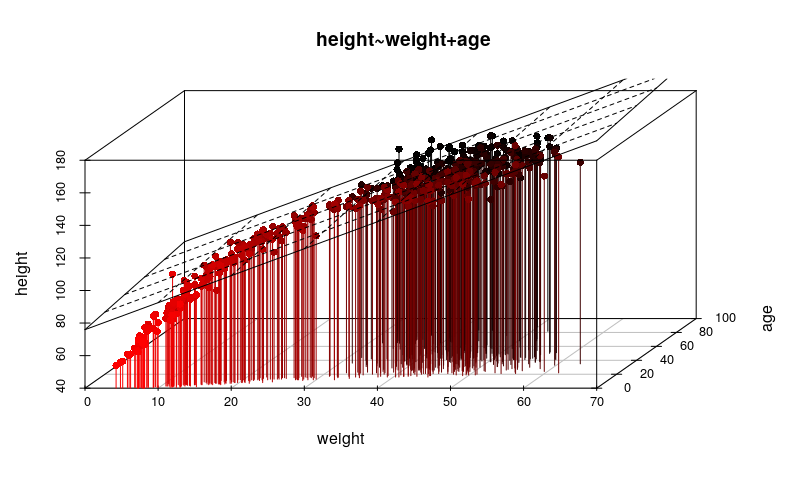
\includegraphics[scale=0.55]{pics/reg3d.png}
\end{figure}
 
\end{frame}


\begin{frame}{$R^2$ adjusted}
 \scriptsize{
 \begin{itemize}
  \item The coefficient of determination $R^2$ tends increases when extra explanatory variables are added to the model.
  
  \item This happens even when the additional variables are useless.
  
  \item This is not desirable a property  when we want to compare different models.

\item $R^2$ adjusted or $\overline{R}^2$ penalizes for the number of variables $m$.
 
\begin{displaymath}
 \overline{R}^2= 1-(1-R^2)\frac{n-1}{n-m-1}
\end{displaymath}

where $n$ is the number of examples.

 \end{itemize}
 }
\end{frame}

\begin{frame}[fragile]{Polynomial Regression}
\scriptsize{ 
\begin{itemize}
 \item Polynomial regression uses powers of a variable (e.g., squares, cubes) as extra attributes.
 
 \item The most common polynomial regression is a parabolic model of the mean:
 
 \begin{displaymath}
 y_i=\beta_{0}+\beta_{1}x_i + \beta_{2}x_i^2 + \epsilon_i \quad \forall i
\end{displaymath}
 
 \item Let's fit a polynomial regression for the height variable using a parabolic model for weight
 
 
 \item Because the square of a large number can be truly massive we are going to standardize the weight by substracting the mean and dividing by the standard deviation.
 
 \begin{verbatim}
  d$weight_s <-(d$weight-mean(d$weight))/sd(d$weight)
 \end{verbatim}

\item Then we fit the model as follows:
\begin{verbatim}
> reg4 <- lm(height~weight_s+I(weight_s^2),d) 
> reg4

Call:
lm(formula = height ~ weight_s + I(weight_s^2), data = d)

Coefficients:
  (Intercept)       weight_s  I(weight_s^2)  
      146.660         21.415         -8.412
\end{verbatim}

 
 
\end{itemize}


}
\end{frame}


\begin{frame}[fragile]{Categorical Predictors}
\scriptsize{ 
\begin{itemize}
 \item We can also add categorical predictors to our model. 
 
 \item For example let's try using the sex of the Kalahari people to predict height: 


  \begin{displaymath}
  \text{height}(\text{male})=\beta_0+\beta_1*\text{male}
 \end{displaymath} 

 \item Here ``male'' is a binary or dummy variable (it takes the value 1 when the person is male and 0 otherwise).
 
 \item In R, it is important to make sure that our categorical variables are represented as factors:
 
 \begin{verbatim}
> d$male<-as.factor(d$male)
> reg5<-lm(height~male,d)
\end{verbatim}

\item The coefficients of the model are:

\begin{verbatim}
> reg5$coefficients
(Intercept)       male1 
 134.630278    7.690759  
\end{verbatim}


 
\end{itemize}





}
\end{frame}


\begin{frame}[fragile]{Categorical Predictors}
\scriptsize{ 
\begin{itemize}
\item Here $\beta_0$ is the average height of females and $\beta_1$ is the average height difference  between males and females:
 
\end{itemize}

\begin{verbatim}
> sum(reg5$coefficients)
[1] 142.321
> means<-tapply(d$height,d$male,mean)
> means
       0        1 
134.6303 142.3210
> means[2]-means[1]
       1 
7.690759 
\end{verbatim}



}
\end{frame}

\begin{frame}[fragile]{Categorical Predictors}
\scriptsize{ 

\begin{verbatim}
> summary(reg5)

Call:
lm(formula = height ~ male, data = d)

Residuals:
   Min     1Q Median     3Q    Max 
-81.87 -12.73  12.65  18.33  36.75 

Coefficients:
            Estimate Std. Error t value Pr(>|t|)    
(Intercept)  134.630      1.615  83.366  < 2e-16 ***
male1          7.691      2.350   3.273  0.00113 ** 
---
Signif. codes:  0 ‘***’ 0.001 ‘**’ 0.01 ‘*’ 0.05 ‘.’ 0.1 ‘ ’ 1

Residual standard error: 27.36 on 542 degrees of freedom
Multiple R-squared:  0.01938,	Adjusted R-squared:  0.01758 
F-statistic: 10.71 on 1 and 542 DF,  p-value: 0.001131
\end{verbatim}



}
\end{frame}


\begin{frame}[fragile]{Categorical Predictors}
\scriptsize{ 
\begin{itemize}
\item The p-value of the statistical sinfificance test for $\beta_1$ in reg5  is the same as that obtained from an unpaired two-sample t-tests with equal variance:
\begin{verbatim}
> t.test(d$height~d$male, var.equal=T)

	Two Sample t-test

data:  d$height by d$male
t = -3.2733, df = 542, p-value = 0.001131
alternative hypothesis: true difference in means is not equal to 0
95 percent confidence interval:
 -12.306146  -3.075372
sample estimates:
mean in group 0 mean in group 1 
       134.6303        142.3210 
 
\end{verbatim}

\item Notice that we must set \verb+var.equal=T+ to get the same results, since the linear model assumes that the variance is constant.


\end{itemize}





}
\end{frame}


\begin{frame}[fragile]{Categorical Predictors}
\scriptsize{ 
\begin{itemize}
\item We can also fit a multivariate linear model with both numeric and categorical variables:
  \begin{displaymath}
  \text{height}(\text{weight,male})=\beta_0+\beta_1*\text{weight}+\beta_2*\text{male}
 \end{displaymath} 

\begin{verbatim}
> reg6<-lm(height~weight+male,d)
> reg6

Call:
lm(formula = height ~ weight + male, data = d)

Coefficients:
(Intercept)       weight        male1  
    75.5489       1.7664      -0.3971  
\end{verbatim} 
 
\item In this model we use the same slope $\beta_1$ relating height to weight for both groups.

\item The coefficient $\beta_2$ indicates an expected weight difference between males and females once the ``weight'' is known.
 
\end{itemize}





}
\end{frame}

\begin{frame}[fragile]{Interactions}
\scriptsize{ 
\begin{itemize}
\item In many cases we want to fit a model using lines with separate slopes for each category.

\item This is done using an \textbf{interaction}, which in our case is just an additional parameter associated with the the product between the category and the predictor.

  \begin{displaymath}
  \text{height}_{int}(\text{weight,male})=\beta_0^{(i)}+\beta_1^{(i)}*\text{weight}+\beta_2^{(i)}*\text{male}+\beta_3^{(i)}*\text{weight}*\text{male}
 \end{displaymath}

\item In R, interactions are denoted by using the * or : symbol in the formula.
\begin{verbatim}
> reg7<-lm(height~weight+male+weight:male,d)
> # or lm(height~weight*male,d)
> reg7

Call:
lm(formula = height ~ weight + male + weight:male, data = d)

Coefficients:
 (Intercept)        weight         male1  weight:male1  
     74.2536        1.8051        2.0683       -0.0695  
\end{verbatim} 
 

\end{itemize}



}
\end{frame}


\begin{frame}[fragile]{Interactions}
\scriptsize{ 
\begin{itemize}
\item The above model can be interpreted as a compact version of fitting two models, one for each group.

\item A model for the male group would be as follows:


  \begin{displaymath}
  \text{height}_{male}(\text{weight}_{male})=\beta_0^{(m)}+\beta_1^{(m)}*\text{weight}_{male}
 \end{displaymath}
 
 \begin{verbatim}
> d.male<-d[d$male==1,]
> reg8<-lm(height~weight,d.male)
Call:
lm(formula = height ~ weight, data = d.male)
Coefficients:
(Intercept)       weight  
     76.322        1.736  
\end{verbatim} 

and for the female group:
 
   \begin{displaymath}
  \text{height}_{female}(\text{weight}_{male})=\beta_0^{(f)}+\beta_1^{(f)}*\text{weight}_{male}
 \end{displaymath}


\begin{verbatim}
> d.female<-d[d$male==0,]     
> reg9<-lm(height~weight,d.female)
Call:
lm(formula = height ~ weight, data = d.female)
Coefficients:
(Intercept)       weight  
     74.254        1.805  
\end{verbatim} 

 
\end{itemize}




}
\end{frame}

\begin{frame}[fragile]{Interactions}
\scriptsize{ 
\begin{itemize}
\item We can find many relationships between the coefficients of the model with interaction  and the two independent models.

\item All of them can be deduced by cancelling out terms in the formula of $\text{height}_{int}$ for the female cases ($male=0$).


\item First, the intercept of the model with the interaction $\text{height}_{int}$ is the same as the intercept of the model for females  $\beta_0^{(i)}=\beta_0^{(f)}$:
\begin{verbatim}
> reg7$coefficients["(Intercept)"]
(Intercept) 
   74.25359 
> reg9$coefficient["(Intercept)"]
(Intercept) 
   74.25359  
\end{verbatim}

\item The same applies for the slope of weight for $\text{height}_{int}$  and  $\text{height}_{female}$    $\beta_1^{(i)}=\beta_1^{(f)}$:
\begin{verbatim}
> reg7$coefficients["weight"]
  weight 
1.805118 
> reg9$coefficient["weight"]
  weight 
1.805118 
\end{verbatim}

 
\end{itemize}





}
\end{frame}



\begin{frame}[fragile]{Interactions}
\scriptsize{ 
\begin{itemize}
\item  The interaction slope from $\text{height}_{int}$  encodes the difference in weight slopes between both groups $\beta_3^{(i)}=\beta_1^{(m)}-\beta_1^{(f)}$:
 
 \begin{verbatim}
> reg7$coefficients["weight:male1"]
weight:male1 
 -0.06949648 
> reg8$coefficient["weight"]-reg9$coefficient["weight"]
     weight 
-0.06949648 
 \end{verbatim}


\item Finally, the category coefficient $\beta_2^{(i)}$  from  $\text{height}_{int}$ corresponds to the difference of intercepts between  $\text{height}_{male}$ and  $\text{height}_{female}$
$\beta_2^{(i)}=\beta_0^{(m)}-\beta_0^{(f)}$: 



\begin{verbatim}
> reg7$coefficients["male1"]
   male1 
2.068278 
> reg8$coefficients["(Intercept)"]
-reg9$coefficient["(Intercept)"]
(Intercept) 
   2.068278  
\end{verbatim}
 
 
 
\end{itemize}





}
\end{frame}


\begin{frame}{Conclusion}
 
 \scriptsize{
 \begin{itemize}
  \item We can use a simple linear model to describe the relation between two variables and to decide whether that relationship is statistically significant.
  
  \item In addition, the model allows us to predict the value of the dependent variable given some new value(s) of the independent variable(s).
  
  \item Most importantly, a mutivariate linear model allow us to build models that incorporate multiple independent variables.
 


 \end{itemize}
 }
 
\end{frame}


\begin{frame}{Bonus: Four Cardinal Rules of Statistics by Daniela Witten}
\scriptsize{

Now that we have concluded the chapter on Frequentist inference, it is good to discuss the points raised by Daniela Witten in a tweet.

\begin{figure}[h!]
	\centering
	
\includegraphics[scale=0.3]{pics/witten.png}
\end{figure}


\begin{block}{One: Correlation does not imply causation}
\begin{itemize}
 \item Yes, I know you know this, but it’s so easy to forget! Yeah, YOU OVER THERE, you with the p-value of 0.0000001 — yes, YOU!! That’s not causation.
 \item No matter how small the p-value for a regression of IQ onto shoe size is, that doesn’t mean that big feet cause smarts!!  It just means that grown-ups tend to have bigger feet and higher IQs than kids.
 \item So, unless you can design your study to uncover causation (very hard to do in most practical settings — the field of causal inference is devoted to understanding the settings in which it is possible), the best you can do is to discover correlations.  Sad but true.
\end{itemize}

 
\end{block}




} 
\end{frame}

\begin{frame}{Bonus: Four Cardinal Rules of Statistics by Daniela Witten}
\scriptsize{


\begin{block}{Two:  a p-value is just a test of sample size}
\begin{itemize}
 \item  Read that again — I mean what I said!  If your null hypothesis doesn't hold (and null hypotheses never hold IRL) then the larger your sample size, the smaller your p-value will tend to be.
 \item If you’re testing whether mean=0 and actually the truth is that mean=0.000000001, and if you have a large enough sample size, then YOU WILL GET A TINY P-VALUE.
 \item Why does this matter? In many contemporary settings (think: the internet), sample sizes are so huge that we can get TINY p-values even when the deviation from the null hypothesis is negligible. In other words, we can have STATISTICAL significance w/o PRACTICAL significance.
 \item Often, people focus on that tiny p-value, and the fact that the effect is of **literally no practical relevance** is totally lost.
 \item This also means that with a large enough sample size we can reject basically ANY null hypothesis (since the null hypothesis never exactly holds IRL, but it might be “close enough” that the violation of the null hypothesis is not important). 
 \item Want to write a paper saying Lucky Charms consumption is correlated w/blood type? W/a large enough sample size, you can get a small p-value.  (Provided there’s some super convoluted mechanism with some teeny effect size… which there probably is, b/c IRL null never holds)
\end{itemize}

 
\end{block}


} 
\end{frame}



\begin{frame}{Bonus: Four Cardinal Rules of Statistics by Daniela Witten}
\scriptsize{


\begin{block}{Three: seek and you shall find}
\begin{itemize}
 \item If you look at your data for long enough, you will find something interesting, even if only by chance! 
 \item  In principle, we know that we need to perform a correction for multiple testing if we conduct a bunch of tests.
\item But in practice, what if we decide what test(s) to conduct AFTER we look at data?  Our p-value will be misleadingly small because we peeked at the data.  Pre-specifying our analysis plan in advance keeps us honest… but in reality, it’s hard to do!!!
\end{itemize}

 
\end{block}


\begin{itemize}
\item Everyone is asking me about the mysterious and much-anticipated fourth rule of statistics. The answer is simple: we haven’t figured it out yet.... that’s the reason we need to do research in statistics
\end{itemize}

} 
\end{frame}

%%%%%%%%%%%%%%%%%%%%%%%%%%%
%%%%%%%%%%%%%%%%%%%%%%%%%%%
\begin{frame}[allowframebreaks]\scriptsize
\frametitle{References}
\bibliography{bio}
\bibliographystyle{apalike}
%\bibliographystyle{flexbib}
\end{frame}  





%%%%%%%%%%%%%%%%%%%%%%%%%%%

\end{document}
